\documentclass[pdf]{beamer}

\mode<presentation>{\usetheme{Warsaw}}
\usecolortheme{dove}

% http://web.mit.edu/rsi/www/pdfs/beamer-tutorial.pdf
% https://rohanverma.net/blog/2017/12/20/setting-up-latex-on-spacemacs/
% begin end CTRL-c CRTL-e

\AtBeginSection[]
{
  \begin{frame}
    \frametitle{Table of Contents}
    \tableofcontents[currentsection, hideothersubsections]
  \end{frame}
}

\usepackage[defaultfam,tabular,lining]{montserrat} %% Option 'defaultfam'
%% only if the base font of the document is to be sans serif
\usepackage[T1]{fontenc}
\renewcommand*\oldstylenums[1]{{\fontfamily{Montserrat-TOsF}\selectfont #1}}

\definecolor{ao(english)}{rgb}{0.0, 0.6, 0.0} % warning: duplicate below
\definecolor{azure(colorwheel)}{rgb}{0.0, 0.5, 1.0} % warning: duplicate below
\newcommand{\green}[1]{\textcolor{ao(english)}{#1}}}
\newcommand{\blue}[1]{\textcolor{azure(colorwheel)}{#1}}}

\newcommand{\pgreen}[1]{\color<#1>[rgb]{0.0, 0.6. 0.0}}}
\newcommand{\pblue}[1]{\color<#1>[rgb]{0.0, 0.5, 1.0}}}

\title{Automatically responding to customers}
\begin{document}

\begin{frame}
  \titlepage
\end{frame}

\begin{frame}
  \frametitle{Table of Contents}
  \tableofcontents[hideothersubsections]
\end{frame}

\section{Introduction}
\subsection{Research question 1}
\begin{frame}{Existing benchmarks}
  \begin{itemize}
  \item Braun et al.
  \item Snips (next slide)
  \item Burtsev et al.
  \item Botfuel
  \end{itemize}
\end{frame}

\begin{frame}{Snips entity recognition}
  \begin{center}
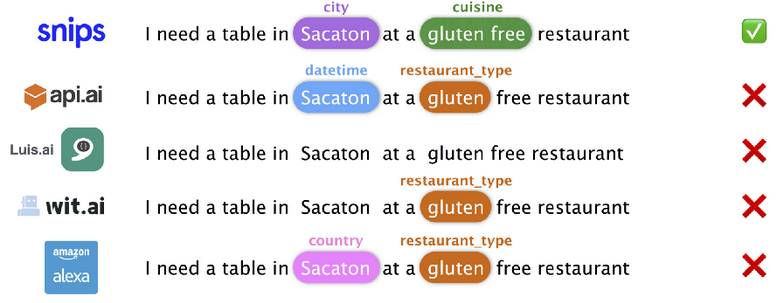
\includegraphics[width=\textwidth]{figures/snips_ner.png}
  \end{center}
\end{frame}

\begin{frame}{Results according to Snips}
  \begin{center}
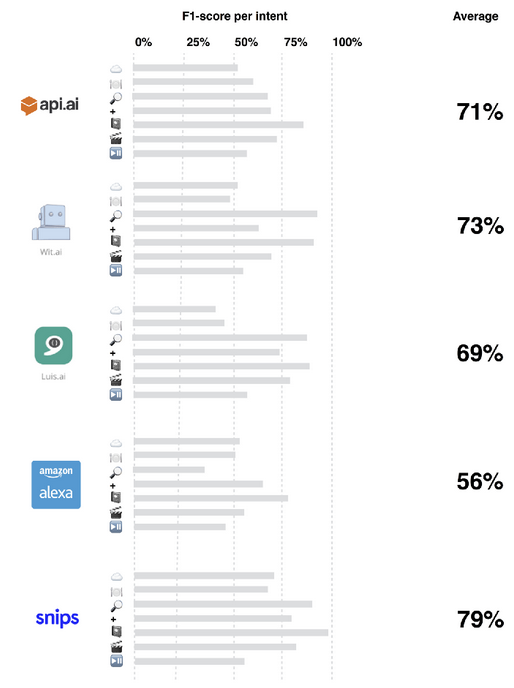
\includegraphics[height=0.85\textheight]{figures/snips_own_benchmark.png}
  \end{center}
\end{frame}

\begin{frame}{Question and goal}
  \begin{itemize}
  \item Can an open-source NLU benchmarking tool be created?
  \item Develop such a tool.
  \end{itemize}
\end{frame}

\subsection{Research question 2}
\begin{frame}{Improving accuracy}
 How hard can it be? 
\end{frame}

\begin{frame}{Question and goal}
  \begin{itemize}
  \item Can accuracy for NLU be increased?
  \item Improve the accuracy
  \end{itemize}
\end{frame}


\section{Preliminaries}
\subsection{Natural language processing}
\begin{frame}{Description of NLP field}
\begin{itemize}
\item Extract meaningful information from
  \begin{itemize}
  \item Text
    \item Speech
  \end{itemize}
\item Generate text
\end{itemize}
\end{frame}

\begin{frame}{Well-known NLP tasks}
  \begin{itemize}
    \item Machine translation
    \item Speech recognition
    \item {\pgreen{2-3}{Named-entity recognition}}
    \item {\pblue{3}{Intent classification}}
    \end{itemize}
    \vspace*{5mm}
    \uncover<2-3>{What is [London's](\green{location}) weather [tomorrow](\green{date})?} \\[3mm]
    \uncover<3>{\blue{get\_weather}}
\end{frame}

\subsection{Deep learning}

\section{Benchmarking}
\subsection{Datasets}
\subsection{Systems}
\subsection{Results}

\section{Improving accuracy}

\section{Conclusions}
\subsection{Research question 1}
\begin{frame}{Research question 1}
\end{frame}

\subsection{Research question 2}
\begin{frame}{Research question 2}

\end{frame}
\end{document}
